\chapter[How fast is light?]{How fast is light?\footnote{Developed by Paolo Privatera 2017, revised by Brent Barker 2021}}

%todo add Greek and Arab theorists to intro

\section{Introduction}

In the early 1600s, the Italian physicist Galileo Galilei was the first to attempt to measure the speed of light with an ingenious experiment. On top of a hill in the beautiful Tuscan country (Fig. \ref{sol:fig:tuscany}), Galileo opened the shutter of his lantern and started a clock (he used his pulse as a timer!).  At the sight of Galileo’s light, an assistant on a nearby hill opened the shutter of his own lantern. Galileo then stopped the “clock” as soon as he saw the light from the assistant’s lantern. He would measure the speed of light as the ratio of twice the distance between the hilltops (the total distance traveled by the light) to the time measured with his “clock”.  Galileo repeated the experiment from various hill tops, and, no matter how far apart they were, he obtained the same time interval, concluding that his method was not accurate enough to measure the speed of light. Indeed, the light time travel was much smaller than the minimum time interval of the  “clock” ($\sim 1\:$s since the pulse rate is $\sim 60$ per minute) and the time measured by Galileo was essentially determined by human reaction time.

\begin{figure}
	\centering
	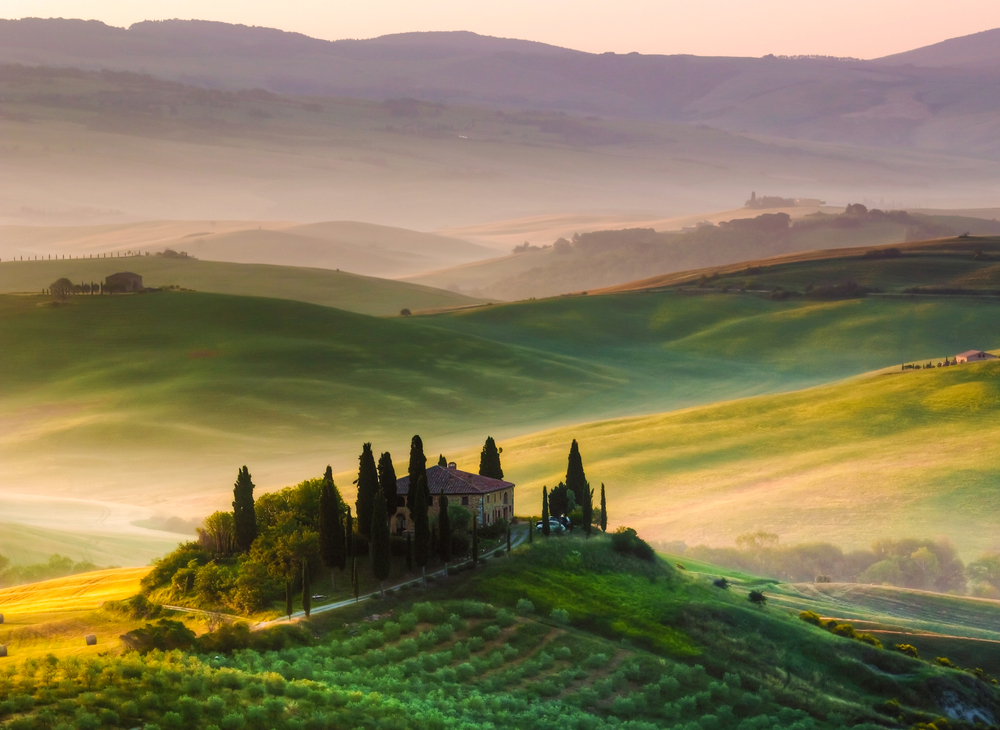
\includegraphics[width=0.5\textwidth]{speed-of-light/tuscany.png}
	\caption{Tuscany Hills}\label{sol:fig:tuscany}
\end{figure}

After Galileo’s first attempt, many ingenious experiments have determined the speed of light with amazing precision (4 parts per billion), including those employing a fast rotating mirror by Albert Michelson, professor at University of Chicago and winner of the Nobel Prize in Physics (1907).   

In this lab, you will measure the speed of light with a method similar to Galileo’s but with some helpful improvements: a mirror will replace Galileo’s assistant (eliminating the delay introduced by his reaction time!) and the time of travel will be measured with nanosecond resolution by an extremely fast light detector.

\section{Forming Groups}

Find your group of 2--3 people. You can change groups from week to week, if you'd like.

\begin{steps}
	\item Once you have a group, meet with each other and decide a) what tools you will use to communicate and collaborate, b) when you will meet, c) what you will do when you need to change an agreement, and d) what you will do when a member has a concern about how the group is functioning. \textbf{Record your agreements.}% This part counts as data collection and analysis, so it can be identical in each member's report.}
\end{steps}

\subsection{Team roles}

\begin{steps}
	\item \textbf{Decide on roles} for each group member.
\end{steps}

The available roles are:
\begin{itemize}
	\item Facilitator: ensures time and group focus are efficiently used
	\item Scribe: ensures work is recorded
	\item Technician: oversees apparatus assembly, usage
	\item Skeptic: ensures group is questioning itself
\end{itemize}

These roles can rotate each lab, and you will report at the end of the lab report on how it went for each role. Some members will be holding more than one role. For example, you could have the skeptic double with another role. Consider taking on a role you are less comfortable with, to gain experience and more comfort in that role.

Additionally, if you are finding the lab roles more restrictive than helpful, you can decide to co-hold some or all roles, or think of them more like functions that every team needs to carry out, and then reflect on how the team executed each function.

\subsection{Add members to Canvas lab report assignment group}

\begin{steps}
	\item On Canvas, navigate to the People section, then to the ``Lab 1 Groups'' tab. Find a group that is not yet used, and have each person in your group add themselves to that same lab group.
\end{steps}

This enables group grading of your lab report. Only one person will submit the group report, and all members of the group will receive the grade and have access to view the graded assignment.

\section{The Scientific Cycle\protect\footnote{adapted from Etkina, Planinsic, Van Heuvelen, College Physics, 2nd ed. (2014)}}

One way of describing science is the process of incrementally improving a shared model of how our universe works. In different fields of science, different methods and cycles are used, so there is no ``One True Scientific Method.'' One can still create a model for the process of science, and we describe here one such cycle (the hypothetico-deductive cycle), summarized in Figure~\ref{me:fig:isle}.

In this cycle, there are three types of experiments, each one representing a different stage of the scientific effort. One stage, often started when encountering a novel phenomenon, is the \textbf{observational experiment}. This is an experiment that consists of deciding what to observe and how to observe it, collecting data, finding a pattern, and brainstorming possible explanations for what is observed (also called ``hypotheses'').

Once one has some trial explanations, one can test one or more of those with a \textbf{testing experiment}. Here, one designs a new experimental procedure and uses each hypothesis to predict what will happen. Then the prediction is compared to the procedure's outcome. If they are different, then the hypothesis is judged to be not a helpful explanation for that phenomenon. If they are the same, then it is still helpful. Throughout this stage, one may make various assumptions that would need to be validated, as they can effect the prediction or outcome.

Once a hypothesis has been tested enough for people to find it useful, then it can be applied to solve practical problems, or to determine properties of particular situations, in an ``application experiment.''

\begin{figure}
	\centering
	\includegraphics[width=0.7\textwidth]{ripple-tank/islegraphic.png}
	\caption{A model of the process some scientists go through to create knowledge.\label{me:fig:isle}}
\end{figure}

\section{Application experiment: measure the speed of light}

\subsection{Goal}

Use the kinematic equations to experimentally determine the speed of light produced by a pulsed laser.

\subsection{Available equipment}

\begin{itemize}
	\item Oscilloscope
	\item Pulsed laser
	\item Photodiode
\end{itemize}

\begin{framed}
	\textbf{Warning: Laser Hazard!} The power of our lasers is low enough that the normal human blink reflex is sufficient to protect against incidental eye exposure.
	
	That being said, the following rules reduce the risk of eye exposure to laser light:
	\begin{enumerate}
		\item Do not direct the laser beam into anyone's eye.
		\item Be aware of the laser reflecting off of mirror-like surfaces and where that beam goes.
		\item Turn off the laser when not in use.
		\item Keep the laser pointing horizontally and near the plane of the table, while keep your eyes above that plane.
		\item To determine whether the laser is on, put your hand or a light-colored object in front of the beam, rather than looking into the laser aperture.
	\end{enumerate}
\end{framed}

\begin{framed}
	\textbf{Self-assessment:} To help you improve your scientific abilities, we provide you with self-assessment rubrics.
	A rubric is a scoring system.
	Self-assessment is determining how well you performed a particular task.
	So, these self-assessment rubrics are designed to help you evaluate your performance while you are designing and performing your experiment.
	
	The complete set of rubrics is available in Appendix~\ref{cha:rubrics}.
	In each lab, your report will be assessed using Rubric F, found in Table~\ref{rubric:f}, as well as 5 additional rubric rows listed in that lab.
	Each week, read through these and use them to evaluate your work as you design and perform the experiment.
	Your instructor will use the same rubrics to determine part of your grade for the lab.
\end{framed}	

\subsection{Rubrics to focus on during this experiment:}

See Appendix~\ref{cha:rubrics} for more details.

\begin{itemize}
\item \textbf{A11:} Graph

\item \textbf{D4:} Is able to make a judgment about the results of the experiment

\item \textbf{G1:} Is able to identify sources of experimental uncertainty

\item \textbf{G2:} Is able to evaluate specifically how identified experimental uncertainties affect the data

\item \textbf{G4:} Is able to record and represent data in a meaningful way

\item \textbf{F1:} Is able to communicate the details of an experimental procedure clearly and completely

\item \textbf{F2:} Is able to communicate the point of the experiment clearly and completely

\end{itemize}

\subsection{Speed of light apparatus}

You will use a \textit{time-of-flight} method to measure the speed of light, as illustrated in Figs. \ref{sol:fig:apparatus-sketch}--\ref{sol:fig:apparatus-photo}.  A red laser diode emits periodic flashes of light of very short duration (few $10^{-9}\:$s).  Each pulse of light is directed toward a distant mirror, placed at a distance $L$ from the laser, where it is reflected back toward a light detector (photodiode) located on top of the laser housing. The speed of the light pulse is given by the distance of travel ($D\approx 2L$) divided by the time $t$ required by the pulse to travel to the distant mirror and back:
\begin{equation}\label{sol:eqn:dvt}
v = c = \frac{2L}{t}
\end{equation}
You will measure the distance $L$ with a measuring tape or meter stick, while the time $t$ is measured with the help of an oscilloscope. The electronic circuit driving the laser generates a voltage pulse coincident in time with the firing of the laser flash (yellow line, CH1). A second voltage pulse (blue line, CH2) is produced by the photodiode when hit by the returning light flash. The time difference between these two voltage pulses gives the time of travel $t$.

\begin{figure}
	\centering
	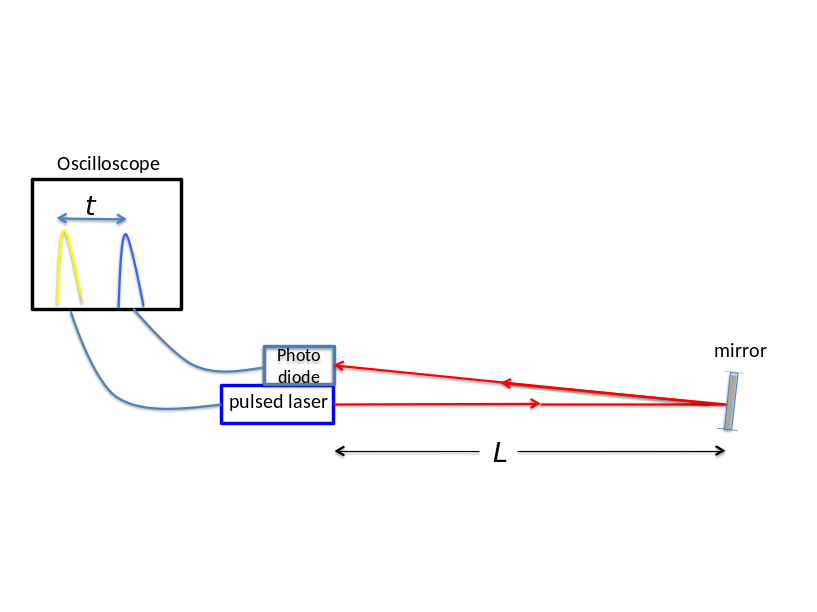
\includegraphics[width=\textwidth]{speed-of-light/apparatus-sketch.png}
	\caption{Sketch of the speed of light apparatus.}\label{sol:fig:apparatus-sketch}
\end{figure}

\begin{figure}
	\centering
	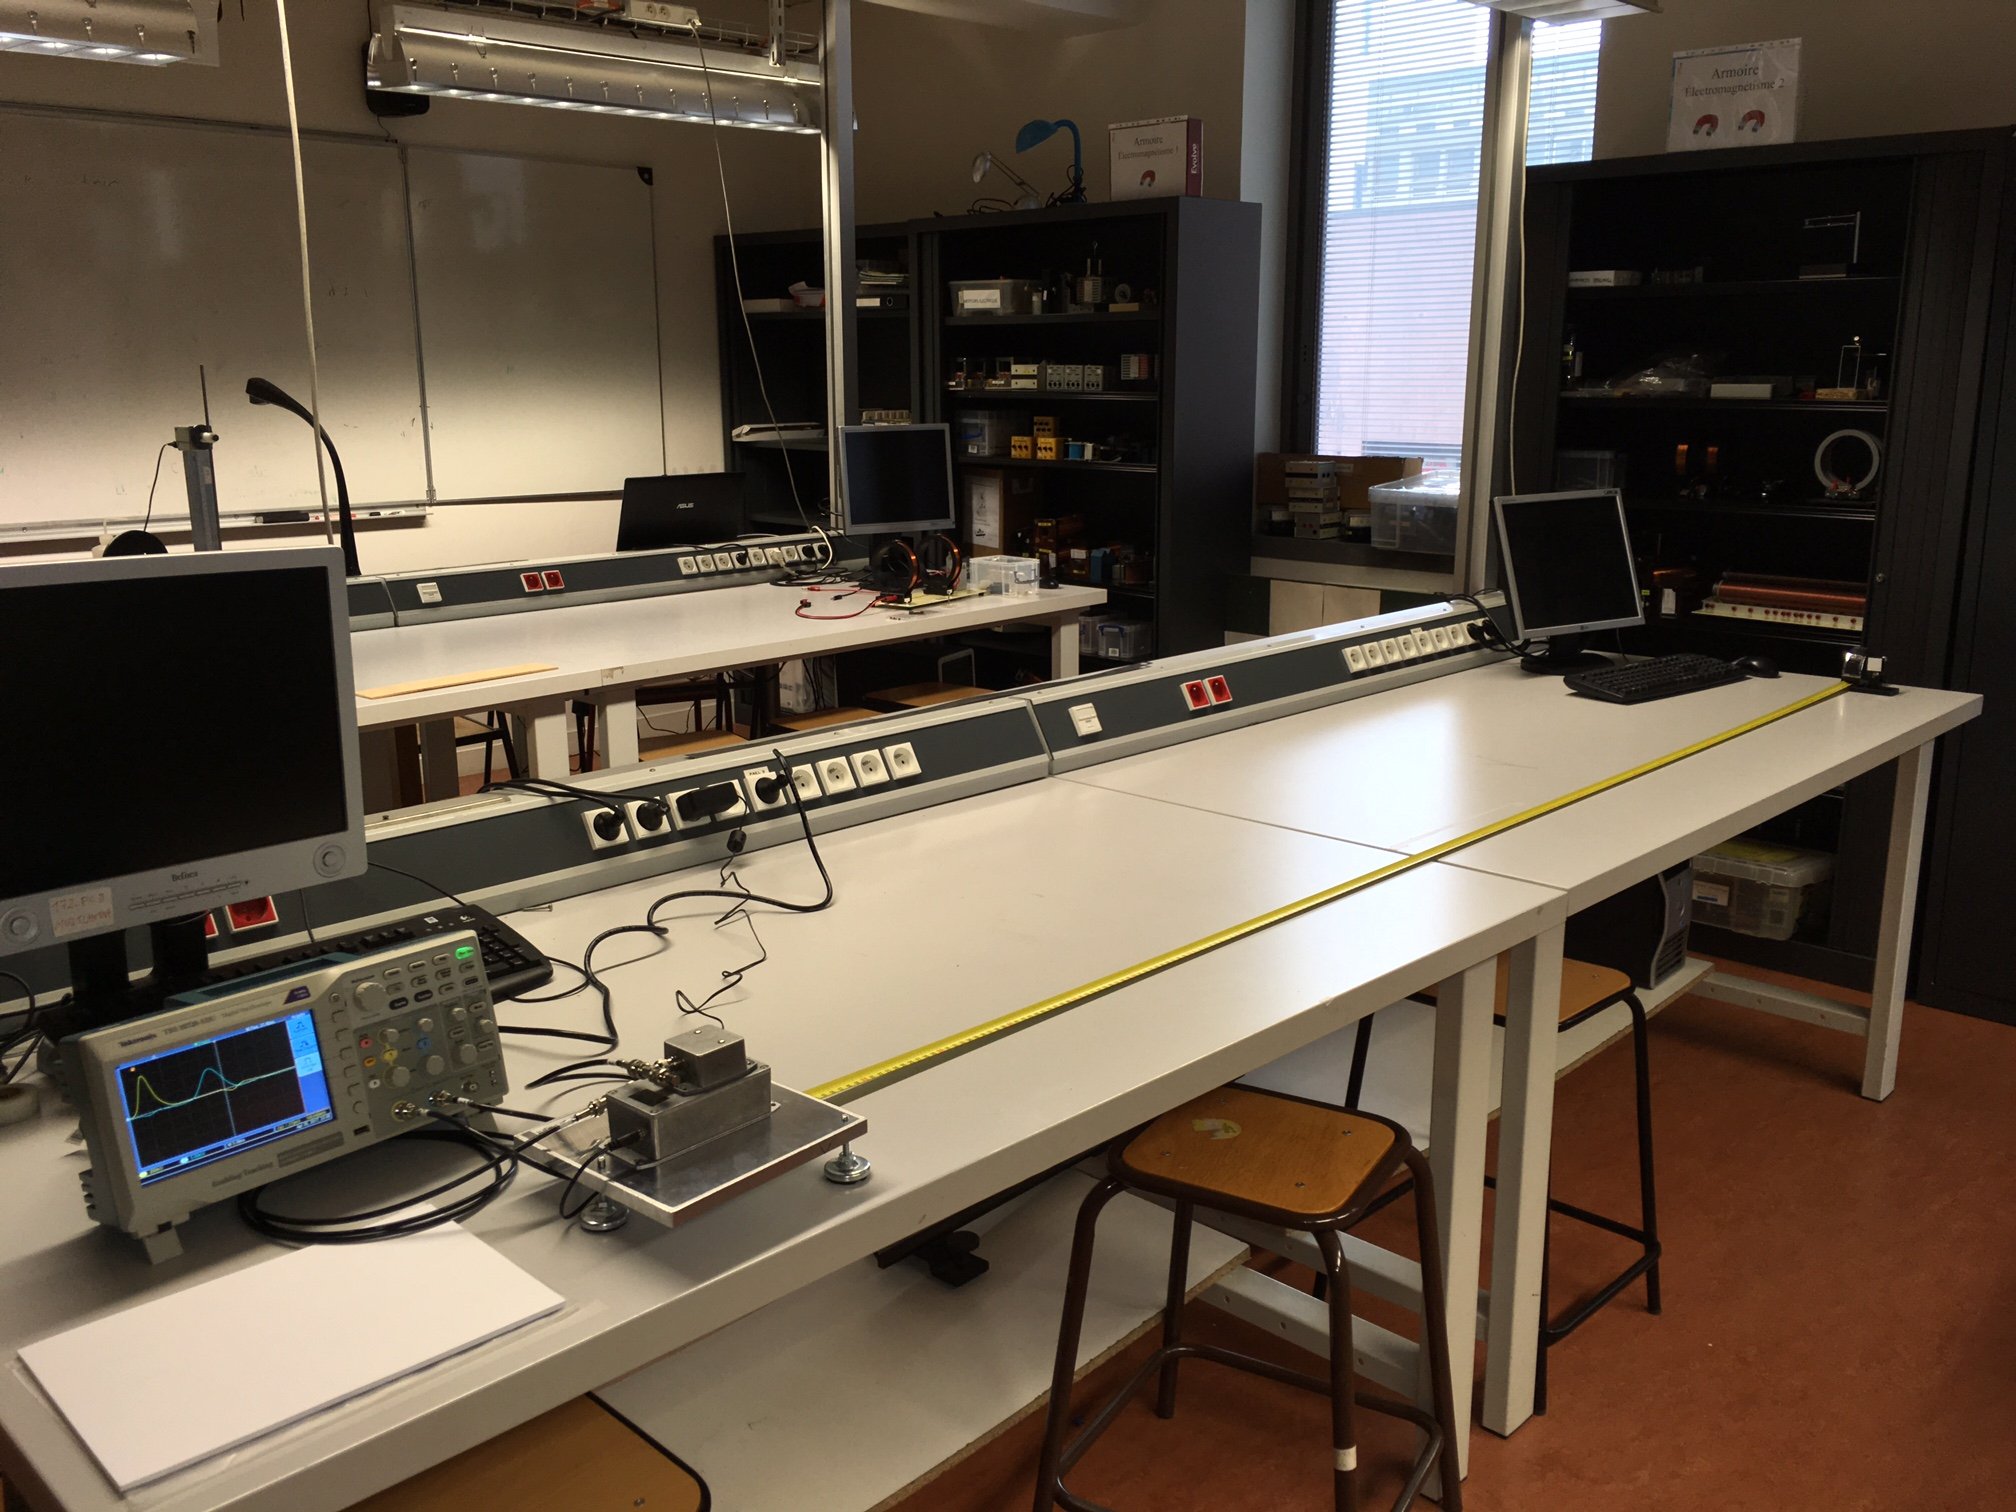
\includegraphics[width=0.8\textwidth]{speed-of-light/apparatus-photo.png}
	\caption{The speed of light setup.}\label{sol:fig:apparatus-photo}
\end{figure}

\subsection{Aligning the mirror}

The alignment of the laser-mirror-photodiode requires a bit of practice but it is not too hard (and is fun!). You will use a sheet of white paper to “catch” the laser spot when doing the alignment.

\begin{steps}
	\item Place the mirror the desired distance from the laser. This is your distance $L$. A useful first distance is 1 meter.
	
	\item Place the white paper at the distance $L$ and see where the laser spot is located. Position the mirror so that the laser spot is approximately at its center (you may have to move the laser base or the mirror vertically.)
	
	\item To catch the reflected laser, slowly move the white paper from the sides (left, right and top with respect to the laser axis) to intercept the laser. Perform this operation with the white paper placed approximately half way between the laser and the mirror. You should find two spots, one of which (the reflected laser beam: “reflected spot”) will disappear when you catch the other (the beam coming directly from the laser: “direct spot”).
	
	\item Once you have identified the reflected spot, move the alignment knobs behind the mirror (slowly, they are very sensitive!) to place it close the direct spot (catching the spots with the white paper will help you during this procedure).  If the reflected spot is too much on the side, you can also rotate the base of the mirror to bring it back along the laser beam axis, and then do the fine adjustments with the mirror alignment knobs.
	
	\item Follow with the white paper the reflected spot back to the laser/photodiode housing. Note that the reflected spot will be quite diffused, particularly for large $L$.
	
	\item By rotating the base of the mirror and/or with small adjustments of the mirror alignment knobs, move the reflected spot so that the photodiode is approximately at its center.  Look at the signal pulse from the photodiode (blue line) and do small adjustment to maximize it so that it is approximately symmetric with a peak height $\ge 15\:$mV.

\end{steps}

\subsection{Observing the signal}

The function of the oscilloscope is to detect a small repeating signal (``oscillation'') and display it in a way useful for analysis. It works at the high frequencies we need (billions of cycles per second, or gigahertz).

\begin{steps}
	\item Be sure that the oscilloscope is setup to display individual pulses (Press “Acquire”, then “Sample”, Figs. \ref{sol:fig:scope-parts} and \ref{sol:fig:scope-average}).

\begin{figure}
	\centering
	\includegraphics[width=0.5\textwidth]{speed-of-light/scope-screen.png}%
	\includegraphics[width=0.5\textwidth]{speed-of-light/scope-commands.png}
	\caption{Left: Oscilloscope screen with Cursor time measurement. Right: Oscilloscope commands.}\label{sol:fig:scope-parts}
\end{figure}

\begin{figure}
	\centering
	\includegraphics[width=0.8\textwidth]{speed-of-light/scope-average.png}
	\caption{Performing Averages with the oscilloscope}\label{sol:fig:scope-average}
\end{figure}

	\item Note the frequency of the periodic flashes as displayed in the lower right corner of the screen. It should be about 100 kHz, since that's the frequency the laser is pulsing at.
	
	\item Expand the time scale by turning the Horizontal Scale knob (see Fig. \ref{sol:fig:scope-parts}, right) and observe that each of these periodic pulses is actually two, closely spaced pulses (Fig. \ref{sol:fig:scope-parts}, left).
	
\end{steps}

The first pulse (yellow line) corresponds to the time when the laser emits the flash, the second pulse (blue line) corresponds to the time of arrival of the light flash at the photodiode.

\subsection{Doing one measurement}

Here you'll actually do a measurement of the speed of light by measuring the distance and time duration and applying Equation\ \ref{sol:eqn:dvt}.

\subsubsection{Measuring distance}

\begin{steps}

	\item With the laser aligned and both pulses visible, measure the mirror distance $L$.

\end{steps}
	
A measurement of a physical quantity is not useful without an estimate of the uncertainty of the measurement.

\begin{steps}
	\item Skim the introduction and Section \ref{unc:sec:types} of Appendix \ref{cha:uncertainty}.
	
	\item Identify some possible sources of uncertainty for the mirror distance measurement. \textbf{Record your answers.}

	\item For each source of uncertainty, decide on the type of uncertainty --- instrumental or random. \textbf{Record your answers.}
	
	\item For each source of uncertainty, estimate the amount of uncertainty. \textbf{Record your answers.}
	
	\item For this measurement, pick the greatest uncertainty from the various sources and ignore the others. Treat this as the uncertainty of this measurement. \textbf{Record your final determination of $L$ and uncertainty $\delta L$.} Express this as $L \pm \delta L$, for example $L = 1.02 \pm 0.01\:$meters.

\end{steps}

\subsubsection{Measuring time}

\begin{steps}

	\item To optimally measure the difference in time between the two pulses, maximize the resolution of the time (Horizontal) scale while keeping both pulses in the screen. The resolution is displayed in the lower middle of the screen, labeled ``M''. Typically you will choose a $5\:$ns/division or $10\:$ns/division in the horizontal scale. Place the source laser pulse (CH1, yellow line) as far left as possible using the Horizontal Position knob so that the full horizontal scale can be used for the measurements.
	
	\item Optimize the photodiode pulse (CH2, blue line) by aligning the laser spot on the photodiode. The resulting pulse should be approximately symmetric with a peak height $\ge 15\:$mV. \textit{Note: always keep the vertical scale of Channel 2 at $\ge 5\:$mV/division, as shown in the lower left marked ``2''.}
	
\end{steps}

Next you will set up the oscilloscope to perform the average of 128 pulses, which will provide improved accuracy in the determination of the position of the pulses.

\begin{steps}
	\item To set the oscilloscope for the average measurement (Fig. \ref{sol:fig:scope-average}), press “Acquire”, then press “Average” and rotate the Multipurpose knob till the number 128 (i.e. average of 128 pulses) is highlighted, and press the Multipurpose knob to select. Press “Menu off” to eliminate the Menu from the screen.
	
\end{steps}

Next you will use the time cursors to measure the time difference $t$ between the peaks of the two pulses.

\begin{steps}
	
	\item Press “Cursor” (Fig. \ref{sol:fig:scope-parts}, right). Check that cursor “Type” is “Time”, then press “Cursor 1” in the Cursor Menu and move the cursor by turning the Multipurpose knob so that it coincides with the peak of the source pulse. Press “Cursor 2” and move the cursor until it coincides with the peak of the detector pulse. The time difference between the two cursors (corresponding to the time of travel $t$) will be displayed as “$\Delta$ .. ns” in the Cursor Menu (third tab from the top). \textbf{Record your measured time difference.}
	
	\item Identify the sources of uncertainty, estimate each of them, choose the largest, and \textbf{record your time difference $t$ and its uncertainty $\delta t$.}

	\item Use Equation \ref{sol:eqn:dvt} to find your measurement of the speed of light $v_c$.

	\item To find the uncertainty in your measured $v_c$, we must propagate the uncertainty from $L$ and $t$. Since the formula involves division of these two variables, use Equation \ref{unc:mult} to find $\delta v_c$. \textbf{Record your calculation of $v_c \pm \delta v_c$}

\end{steps}

It is okay if this measurement is much different from the standard value of $c \approx 3 \times 10^8\:$m/s. We will examine a possible reason for this in the next section. It should be within a factor of 2 or so at this point. If not, check with your instructor.

\begin{steps}

	\item Press “Acquire”, then “Sample”. This will return the oscilloscope to display individual pulses.

\end{steps}

\section{Checking assumptions}

In our model of the scientific cycle, sources of uncertainty are ones that are quantifiable --- we can estimate the effect and include it as an interval within which we are confident. We use \textit{assumption} to mean things that we are assuming are true that, if not true, would change our result in ways that we cannot or are not estimating. Some assumptions are more about troubleshooting --- for example, we assume that the oscilloscope is working as expected. Others are about our measurement technique. For example, there is a vertical distance between the laser source and the detector. This means that the path the light travels is not simply $2L$.

\begin{steps}
	
	\item By assuming the path the light travels is $2L$, will you over- or under-estimate value of $c$, compared with using a more accurate length? \textbf{Record your answer.}
	
	\item Estimate how much your measurement of the speed of light will change if you use the correct value for the return path (note: the distance between the laser and the photodiode is $4\:$cm). For simplicity, make your estimate only for the measurement where the mirror was at the maximum distance. Do you think this is a small or large effect? \textbf{Record your answers.}
	
\end{steps}

Another assumption is that the lag time from detector to oscilloscope and from source to oscilloscope is the same. That is, the time difference recorded in the oscilloscope includes the time for the signals from the laser and detector to reach it. Since we are talking about time differences on the  order of nanoseconds, small differences in cable length, for example, could change things.

This fixed difference in length $d_e$ is the same no matter the mirror distance $D=2L$. In fact, it should be the same error in length every time. So the recorded time difference $t$ would actually be 
\begin{eqnarray}
\textrm{total distance} &=& vt \\
2L + d_e &=& v t \\
2L &=& v t - d_e
\end{eqnarray}

Notice that the last equation is in the same form as that of a straight line, $y = mx + b$. So if we take a series of measurements of $t$ for different distances $2L$, and plot $2L$ vs. $t$, then the slope of the graph will be the speed of light $v$, and that effective length difference $d_e$ will be the $y$-intercept.

\begin{steps}

	\item Measure the time difference for at least 5 different mirror distances, \textbf{recording your measurement in a table}, including the distance $L$ between the laser and the mirror that you have measured with the measuring tape or meter stick. See Table \ref{sol:tab:data} for a sample table format.

\begin{table}
	\centering
	\begin{tabular}{|c|c|c|}
		\toprule
		length (m) & distance $= 2L$ (m) & time ($10^{-9}\:$s) \\
		\midrule
		\ldots & \ldots & \ldots \\
		\bottomrule
	\end{tabular}
	\caption{Sample data collection table.}\label{sol:tab:data}
\end{table}

	\item Once your measurements are completed, graph the data of your table in a plot with time of travel $t$ in the horizontal axis and distance of travel ($D = 2L$) in the vertical axis.
	
	\item To determine the speed of light $c$, fit your data with a line (e.g. with Excel by displaying your data with Scatter, and then using Trendline;  select 'Display Equation on Chart' in Trendline Options). The slope of the line will be your estimate of the speed of light. (NOTE: pay attention to the units). \textbf{Take a screenshot of your graph for your report.}
	
\end{steps}
	
In this case, to determine the uncertainty, you will not use the uncertainty of each individual point. Instead, you will use the coefficient of determination, $r^2$, which is given by your plotting program, along with the number of data points you took, $N$, to find the uncertainty, which is the standard error $SE$ of the slope $m$, given as
\begin{equation}\label{sol:eqn:sem}
SE(m) = m \sqrt{\frac{1-r^2}{r^2 (N-2)}}
\end{equation}

\begin{steps}

	\item Find the uncertainty in the speed of light measurement using Equation \ref{sol:eqn:sem}. \textbf{Record your new determination of $c$, with its uncertainty.}
	
	\item Compare your result with the known value of the speed of light, $299\:792\:458\:$m/s. To compare, use the $t'$ statistic as described in Appendix \ref{unc:sec:comparing}.

\end{steps}

\section{Revisiting Galileo's technique}

\begin{steps}
	
	\item Measure your reaction time with a stopwatch (highly likely you have one in your cell phone, or ask the instructor if you need one).  Start-stop the stopwatch and record the time. Take 10 measurements and calculate their average as an estimate of your reaction time.\textbf{Record your results.}
	
	\item Now, imagine you  climb on top of a hill in beautiful Tuscany and shoot a laser pulse (by pressing a button at the same time of the start in the stopwatch) towards a mirror placed $2\:$km away. You press the stop in the stopwatch as soon as you see the returning laser pulse. Would you be able to measure the speed of light? (Calculate the time of travel of the laser pulse and compare it with your reaction time). \textbf{Record your answer and calculation.}
	
	\item At what distance should the mirror be placed for you to be able to measure the speed of light (say with a 20\% uncertainty) using the stopwatch? \textbf{Record your answer.}

\end{steps}

\section{Group dynamics}

\begin{steps}
	\item Write a 100--200 word paragraph reporting back from each of the four roles: facilitator, scribe, technician, skeptic. Where did you see each function happening during this lab, and where did you see gaps? What successes and challenges in group functioning did you have? What do you want to do differently next time?
\end{steps}

\section{Report checklist and grading}

The lab grade consists of 3 points for each of seven scientific ability rubric rows (the 5 listed above, as well as F1 and F2, applied to the entire report), 3 points for attendance and participation, and 6 points for providing evidence in the lab report of completing all steps of the lab, including answering every question, for a total of 30 points.